\documentclass[11pt,a4paper]{book}
\usepackage[utf8]{inputenc}
\usepackage[english]{babel}
\usepackage{amsmath}
\usepackage{amsfonts}
\usepackage{amssymb}
\usepackage{graphicx}
\usepackage{url}
\usepackage{python}
\usepackage{algpseudocode,algorithm}
\usepackage{tikz}
%\usepackage{todonotes}
\usepackage{makeidx}
\usepackage{enumitem}
\usepackage{array}
\usepackage{makecell}
\usepackage{xcolor}

\newcommand\todo[1]{\textcolor{red}{#1}}
\newcommand{\locpath}{..}

\usepackage[left=2.5cm,right=2.5cm,top=2cm,bottom=2.5cm]{geometry}

% Thesis title
%\title{Energy Efficiency, Exascale and Complex Systems}
\title{Vers l'Exascale: Des Probl\`emes Th\'eoriques aux Probl\`emes Appliqu\'es\\
The Way to Exascale: From Theorics to Applied Problems}
% Author
\author{Julien Loiseau}
% Date 
\date{\today}

\makeindex

\begin{document}
\setcounter{chapter}{0}

%%%%%%%%%%%%%%%%%%%%%%%%%%%%%%%%%%%%%%%%%%%%%%%%%%%%%%%%%%%%%%%%%%%%%
%                                                                   %
%	CHAPTER ONE, CHOICES AND SPH                                    %
%                                                                   %
%%%%%%%%%%%%%%%%%%%%%%%%%%%%%%%%%%%%%%%%%%%%%%%%%%%%%%%%%%%%%%%%%%%%%
\chapter{General problem}

\section{Introduction}
In this section we give details on our choices for the generic application confronted to both computation and communication walls in irregular context. 
This problem, the Smoothed Particle Hydrodynamics method implementation, is described on the physics aspect and the difficulties involved in the resolution on supercomputers and accelerators.  

\section{Smoothed Particle Hydrodynamics}

\subsection{General description}
Smoothed Particle Hydrodynamics (SPH) is an explicit numerical mesh-free Lagrangian method.
It is used to solve hydrodynamical partial differential equations (PDEs) by discretized them into a set of fluid elements called particles. 
This computational method was invented for the purpose of astrophysics simulations by Monaghan, Gingold and Lucy in 1977 \cite{lucy1977numerical,gingold1977smoothed}. 
This first SPH work conserved mass and they later proposed a method which also conserves linear and angular moment \cite{gingold1982kernel}. 
The method was extended for general fluid simulation and many more fields from ballistics to oceanography.
The development of new reliable, parallel and distributed tools for this method is a challenge for future HPC architectures with the upcoming Exascale systems.

\begin{figure}
\centering
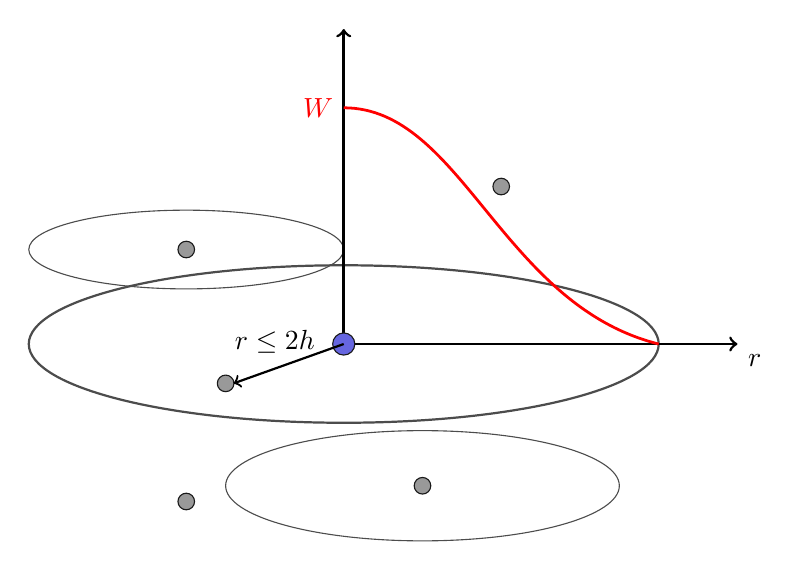
\begin{tikzpicture}
	
	% Others and their ellipse
	\draw [black!90,fill=black!40] (.5,1.5) circle (.3em);
	\draw [black!90,fill=black!40] (0,0) circle (.3em);
	\draw [black!90,fill=black!40] (0,3.2) circle (.3em);
	\draw[black!70] (0,3.2) ellipse (2 and .5);
	\draw [black!90,fill=black!40] (3,.2) circle (.3em);
	\draw[black!70] (3,.2) ellipse (2.5 and .7);
	\draw [black!90,fill=black!40] (4,4) circle (.3em);
	% Ellipses 
	\draw[line width=.8pt,black!70] (2,2) ellipse (4 and 1);
	% Axes
	\draw[->,line width=1pt] (2,2) -- (7,2) node[anchor=north west] {$r$};
	\draw[->,line width=1pt] (2,2) -- (2,6);
	% bezier for kernel 
	\draw[red,line width=1pt]  (6,2) .. controls (4,2.5) and (3.5,5) .. (2,5) node[red,anchor=east] {$W$};
	% main particle, at the end to cover
	\draw [black!90,fill=black!20!blue!60] (2,2) circle (.4em);
	% Arrows 
	\draw[->,line width=.8pt] (2,2) -- (.6,1.5) node[midway, above,xshift=-.5em] {$r\leq2h$};
\end{tikzpicture}
%\includegraphics[scale=.4]{\locpath/figures/flecsph/sph.pdf}
\caption{SPH kernel $W$ and smoothing length $h$ representation}
\label{fig:sph_base}
\end{figure}

The method, as illustrated in figure~\ref{fig:sph_base}, computes the evolution of physical quantities for every particle regarding its neighbors in the radius of its smoothing length $h$. 
The particles in this radius are then valued according to their distance using a smoothing function $W$, also called a kernel. 
The fundamental SPH formulation for any physical quantity $A$ is then to compute with all the neighbors of $b$ of a particle by:
\begin{equation}
A(\vec{r}) \simeq \sum_b \frac{m_b}{\rho_b} A(\vec{r}_b) W ( |\vec{r}-\vec{r}_b|,h)
\end{equation}

On a physics aspect, this method has several advantages:
It can handle deformations, low densities, vacuum, and makes particle tracking easier. 
It also conserves mass, linear and angular momenta, and energy by its construction that implies independence of the numerical resolution. 
Another strong benefit of using SPH is its exact advection of fluid properties. 
Furthermore, the particle structure of SPH easily combines with tree methods for solving Newtonian gravity through N-body simulations.
As a mesh-free method, it avoids the need of grid to calculate the spatial derivatives. 

However, there are cons to consider using SPH: 
It is restricted to low-order rate of convergence on certain PDE formulations; 
It requires careful setup of initial distribution of particles; 
Further, it can be struggle to resolve turbulence-dominated flows and special care must be taken when handling high gradients such as shocks and surface structure of neutron stars.
Many works are leading to handle more cases and to push the limitations of this method \cite{dai2017dual,lind2016incompressible,ren2016dual}.

In this work, we are solving Lagrangian conservation equations (Euler equations) for mass, energy and momentum of an ideal fluid ~\cite{Landau1959}  such that:
\begin{equation}
\frac{d \rho}{d t} = - \rho \nabla \cdot \vec{v}, \quad
\frac{d u}{d t} = \left( \frac{P}{\rho^2} \right) \frac{d \rho}{d t}, \quad
\frac{d \vec{v}}{d t} = - \frac{\nabla P}{\rho}
\end{equation}
with $\rho$ the density, $P$ the pressure, $u$ the internal energy and $v$ the velocity, where $d/dt = \partial_t + \vec{v} \cdot \nabla$ which is convective derivative.

By using the volume element $V_b = m_b / \rho_b$, we can formulate the Newtonian SPH scheme~\cite{rosswog2009} such that
\begin{equation}
\label{eq:rho}
\rho_a = \sum_b m_b W_{ab} (h_a)
\end{equation}
\begin{equation}
\frac{d u_a}{dt} = \frac{P_a}{\rho_a^2} \sum_b m_b \vec{v}_{ab} \cdot \nabla_a W_{ab} 
\end{equation}
\begin{equation}
\frac{d \vec{v}_a}{d t} = - \sum_b m_b \left(\frac{P_a}{\rho_a^2} + \frac{P_b}{\rho_b^2} \right) \nabla_a W_{ab}
\end{equation}
where $W_{ab} = W(| \vec{r}_a - \vec{r}_b |,h)$ is the smoothing kernel. 
The equations we would like to solve allow for emergence of discontinuities from smooth initial data. 
At discontinuities, the entropy increases in shocks. That dissipation occurs inside the shock-front. 
The SPH formulation here is inviscid so we need to handle this dissipation near shocks. 
There are a number of way to handle this problem, but the most widespread approach is to add artificial viscosity (or artificial dissipation) terms in SPH formulation such that:
\begin{equation}
\left(\frac{d u_a}{dt} \right)_{art} = \frac{1}{2} \sum_b m_b \Pi_{ab} \vec{v}_{ab} \cdot \nabla_a W_{ab}
\end{equation}
\begin{equation}
\left(\frac{d\vec{v}_a}{dt} \right)_{art} = - \sum_b m_b \Pi_{ab}\nabla_a W_{ab}
\end{equation}
In general, we can express the equations for internal energy and acceleration with artificial viscosity
\begin{equation}
\label{eq:intern}
\frac{d u_a}{dt} = \sum_b m_b \left(\frac{P_a}{\rho_a^2} + \frac{\Pi_{ab}}{2} \right) \vec{v}_{ab} \cdot \nabla_a W_{ab}
\end{equation}
\begin{equation}
\label{eq:velo}
\frac{d \vec{v}_a}{d t} = - \sum_b m_b \left(\frac{P_a}{\rho_a^2} + \frac{P_b}{\rho_b^2} + \Pi_{ab} \right) \nabla_a W_{ab}
\end{equation}
$\Pi_{ab}$ is the artificial viscosity tensor. 
As long as $\Pi_{ab}$ is symmetric, the conservation of energy, linear and angular momentum is assured by the form of the equation and antisymmetry of the gradient of kernel with respect to the exchange of indices $a$ and $b$. $\Pi_{ab}$ may define different way but here we use~\cite{Monaghan1983} such as: 
\begin{equation}
\Pi_{ab} = \begin{cases}
\frac{- \alpha \bar{c}_{ab} \mu_{ab} + \beta \mu_{ab}^2}{\bar{\rho}_{ab}} & \text{for $\vec{r}_{ab} \cdot \vec{v}_{ab} < 0$} \\
0 & \text{otherwise}
\end{cases}
\end{equation}
\begin{equation}
\mu_{ab} = \frac{\bar{h}_{ab} \vec{r}_{ab} \cdot \vec{v}_{ab}}{r^2_{ab} + \epsilon \bar{h}_{ab}^2}
\end{equation}

Using the usual form $c_s$ as $c_s = \sqrt{\frac{\partial p}{\partial \rho}}$.
The values of $\epsilon$, $\alpha$, and $\beta$ have to be set regarding the problem targeted. 
Here, we use $\epsilon = 0.01h^2$, $\alpha = 1.0$, and $\beta = 2.0$. 

There are many possibilities for the smoothing function, called the kernel. 
As an example the Monaghan's cubic spline kernel is given by:
\begin{equation}
W(\vec{r},h) = \frac{\sigma}{h^D} \begin{cases}
1-\frac{3}{2} q^2 + \frac{3}{4} & \text{if} \indent 0 \leq q \leq 1 \\
\frac{1}{4} (1-q)^3  & \text{if} \indent 1 \leq q \leq 2 \\
0 & \text{otherwise}
\end{cases}
\end{equation}
where $q = r/h$, $r$ the distance between the two particles, $D$ is the number of dimensions and $\sigma$ is a normalization constant with the values:
\begin{equation}
\sigma =  \begin{cases}
\frac{2}{3} & \text{for 1D}  \\
\frac{10}{7 \pi} & \text{for 2D} \\
\frac{1}{\pi} & \text{for 3D}
\end{cases}
\end{equation}

To sum up, the SPH resolution scheme and its routines are presented on algorithm \ref{alg:sph}.
The Equation of State (EOS) and the integration are problem dependent and will be define for each test case in section \ref{sec:applications}. 

\begin{algorithm}
\caption{SPH loop algorithm}\label{alg:sph}
\begin{algorithmic}[1]
\While{not last step}
\State Compute density for each particle (\ref{eq:rho})
\State Compute pressure using EOS 
\State Compute acceleration from pressure forces (\ref{eq:velo})
\State Compute change of internal energy for acceleration (\ref{eq:intern})
\State Advance particles after integration
\EndWhile
\end{algorithmic}
\end{algorithm}

The main downside for the implementation of this method is the requirement for local computation on every particle. 
The particles have to be grouped locally to perform the computation of (\ref{eq:rho}), (\ref{eq:intern}) and (\ref{eq:velo}).
A communication step is needed before and after (\ref{eq:rho}) to get the local physical data to be able to compute (\ref{eq:intern}) and (\ref{eq:velo}).
The tree data structure allows us to perform $O(Nlog(N))$ neighbor search but also add a domain decomposition and distribution layer.

As the SPH method is used in a large panel of fields from astrophysics to fluid mechanic, there are numerous related works. 
We can cite a code developed in the LANL, 2HOT \cite{warren20132hot} that introduced the Hashed Oct Tree structure used in our implementation. 
There is also GADGET-2 \cite{springel2005cosmological}, GIZMO \cite{hopkins2014gizmo} and the most recent publication is GASOLINE \cite{wadsley2017gasoline2} based on PKDGRAV, a specific tree+gravity implementation. 
Several implementations already implement GPU code and tree construction and traversal, one can cite GOTHIC \cite{miki2017gothic}, presenting gravitational tree code accelerated using the latest Fermi, Kepler and Maxwell architectures. But a lot of GPU accelerated work still focused on fluid problems and not on astrophysical problems  \cite{harada2007smoothed,crespo2011gpus}.
We also note that these implementations focus on SPH problems and does not provide a general purpose and multi-physics framework like we intent to provide through FleCSPH and FleCSI. 

\subsection{Gravitation}
For classical problems like fluid flow the gravitation can directly be applied on the particles with the force:
\begin{equation}
	\vec{a_g} = m\vec{g}
\end{equation}

In order to consider astrophysics problems we need to introduice self-gravitation. 
Each particle imply an action on the others base on its distance and mass. 
The equation of gravitation for a particle $i$ with $j$ other particles is: 
\begin{equation}
	\vec{f_a}_i = \sum_j -G \frac{m_i m_j}{|\vec{r_i}-\vec{r_j}|^3} \vec{r_{ij}}
	\label{eq:gravitation}
\end{equation}

This computation involve an $O(N^2)$ complexity and thus is not applicable directly. 
We applied the method called Fast Multipole Method, FMM and discussed in \cite{beatson1997short}.
In this method we compute the gravitation up a approximations. 
The user can refine those approximation changing parameters. 

\begin{figure}
\resizebox {\columnwidth} {!} {
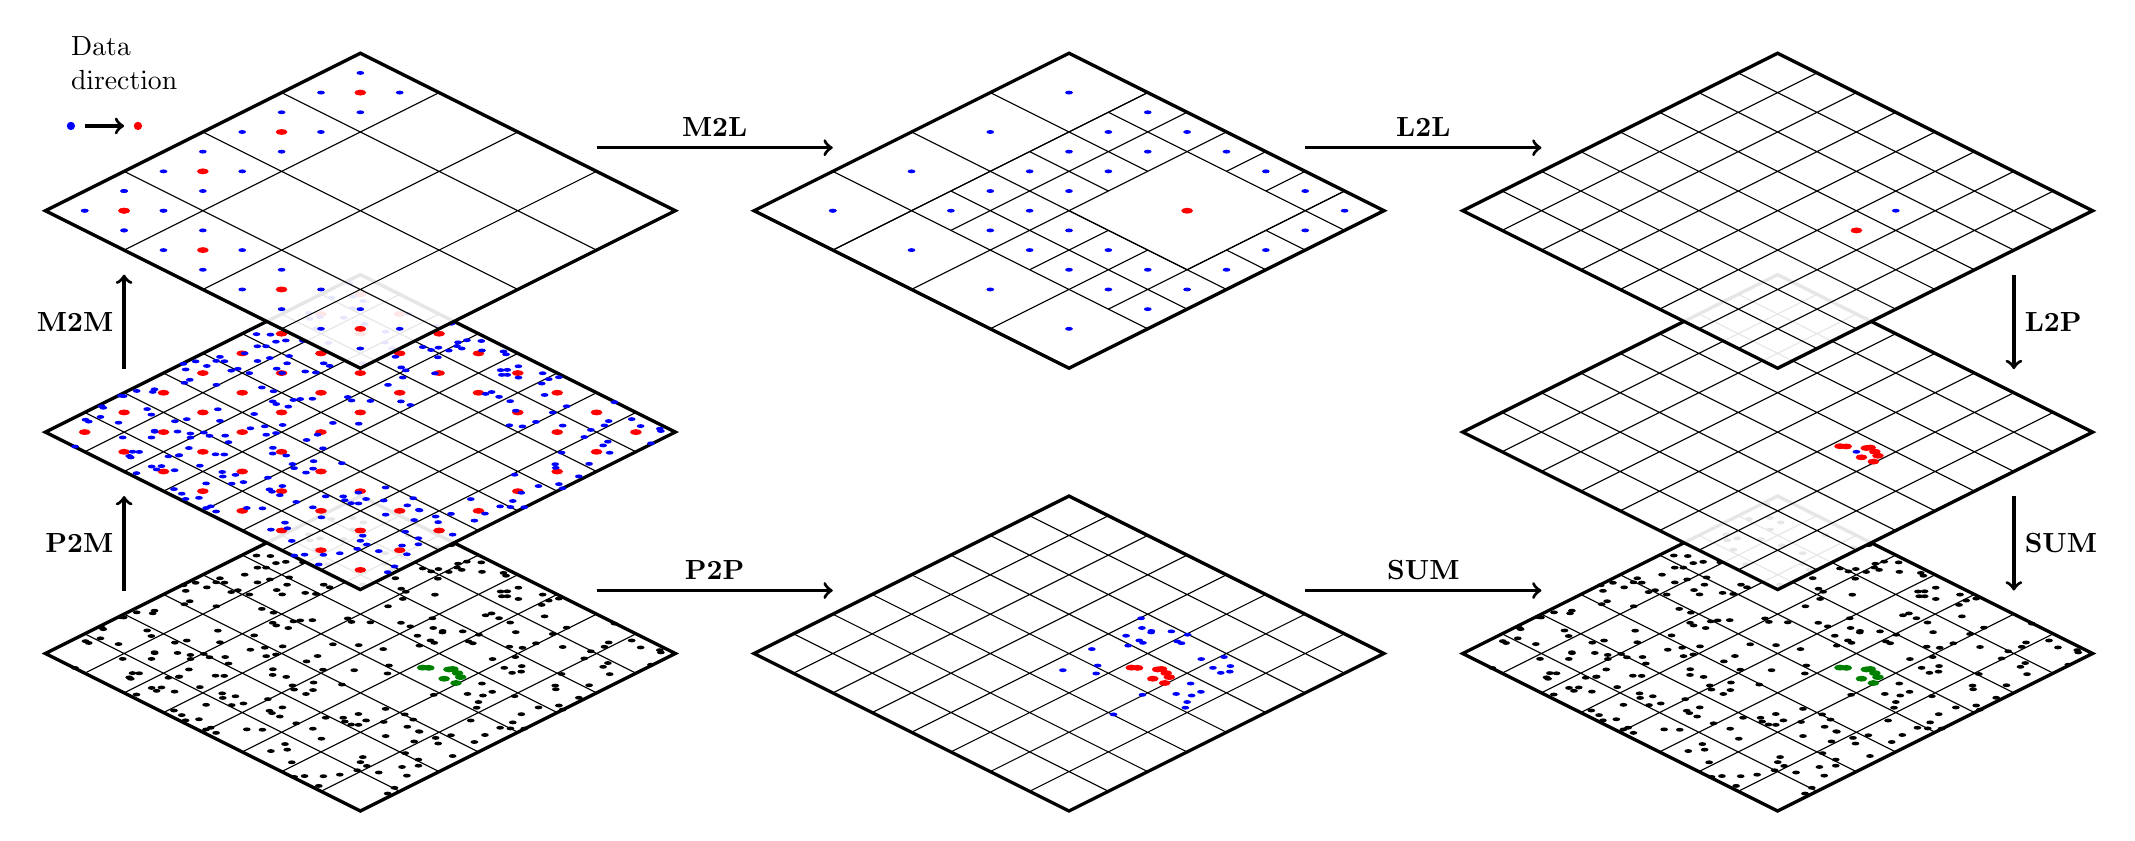
\begin{tikzpicture}
\def\nrand{300}
\def\seed{12}
\def\gridSize{5mm}
\def\gridTotal{4}
% Particles to Multipole
\pgfmathsetseed{\seed}
\begin{scope}[
   		yshift=0,every node/.append style={
    		yslant=0.5,xslant=-1},yslant=0.5,xslant=-1
    ]
    \fill[white,fill opacity=.9] (0,0) rectangle (4,4);
    \draw[black,very thick] (0,0) rectangle (4,4);
	\draw[step=\gridSize, black] (0,0) grid (\gridTotal,\gridTotal);
	\foreach \i in {1,2,...,\nrand}{
    	\pgfmathsetmacro{\x}{(rand)*2+2}
    	\pgfmathsetmacro{\y}{(rand)*2+2}
		% COLOR 
		\ifthenelse{\( \lengthtest{\x cm>2cm} \AND \lengthtest{\x cm<2.5cm} \)}
		{	
			\ifthenelse{ \( \lengthtest{\y cm>1cm} \AND \lengthtest{\y cm<1.5cm} \)}
			{\node at (\x,\y) [black!50!green,circle,fill,inner sep=.7pt,minimum size=3pt]{};}
			{\node at (\x,\y) [circle,fill,inner sep=.7pt]{};}
		}
		{\node at (\x,\y) [circle,fill,inner sep=.7pt]{};}
	}
\end{scope}
\pgfmathsetseed{\seed}
\begin{scope}[
   		yshift=80,every node/.append style={
    		yslant=0.5,xslant=-1},yslant=0.5,xslant=-1
    ]
    \fill[white,fill opacity=.9] (0,0) rectangle (4,4);
    \draw[black,very thick] (0,0) rectangle (4,4);
	\draw[step=5mm, black] (0,0) grid (\gridTotal,\gridTotal);
	\foreach \x in {0,1,...,7}{\foreach \y in {0,1,...,7}{
		\ifthenelse{\( \x<3 \OR \x>5 \)}
		{
			\node at (\x*\gridSize+\gridSize/2,\y*\gridSize+\gridSize/2)[red,circle,fill,inner sep=.7pt,minimum size=3pt]{};
		}
		{	\ifthenelse{ \( \y<1 \OR \y>3 \)}
			{
			\node at (\x*\gridSize+\gridSize/2,\y*\gridSize+\gridSize/2)[red,circle,fill,inner sep=.7pt,minimum size=3pt]{};	
			}{}
		}
	}}
	\foreach \i in {1,2,...,\nrand}{
    	\pgfmathsetmacro{\x}{(rand)*2+2}
    	\pgfmathsetmacro{\y}{(rand)*2+2}
    	\ifthenelse{\( \lengthtest{\x cm<1.5cm} \OR \lengthtest{\x cm>3cm} \)}
		{\node at (\x,\y) [blue,circle,fill,inner sep=.7pt]{};}
		{	\ifthenelse{ \( \lengthtest{\y cm<.5cm} \OR \lengthtest{\y cm>2cm} \)}
			{\node at (\x,\y) [blue,circle,fill,inner sep=.7pt]{};}
			{}
		}
  	}
\end{scope}
\begin{scope}[
   		yshift=160,every node/.append style={
    		yslant=0.5,xslant=-1},yslant=0.5,xslant=-1
    ]
    \fill[white,fill opacity=.9] (0,0) rectangle (4,4);
    \draw[black,very thick] (0,0) rectangle (4,4);
	\draw[step=10mm, black] (0,0) grid (4,4);
	\foreach \x in {0,1}{\foreach \y in {0,...,7}{
		\node at (\x*\gridSize+\gridSize/2,\y*\gridSize+\gridSize/2)[blue,circle,fill,inner sep=.7pt]{};
	}}
	\foreach \x in {0,...,7}{\foreach \y in {6,7}{
		\node at (\x*\gridSize+\gridSize/2,\y*\gridSize+\gridSize/2)[blue,circle,fill,inner sep=.7pt]{};
	}}

	\foreach \x in {0}{\foreach \y in {0,...,3}{				  
		\node at (\x*\gridSize*2+\gridSize,\y*\gridSize*2+\gridSize) [red,circle,fill,inner sep=.7pt,minimum size=3pt]{};
	}}
	\foreach \x in {0,...,3}{\foreach \y in {3}{				  
		\node at (\x*\gridSize*2+\gridSize,\y*\gridSize*2+\gridSize) [red,circle,fill,inner sep=.7pt,minimum size=3pt]{};
	}}
\end{scope}

%PARTICLES TO PARTICLES
\pgfmathsetseed{\seed}
\begin{scope}[
   		yshift=0,xshift=9cm,every node/.append style={
    		yslant=0.5,xslant=-1},yslant=0.5,xslant=-1
    ]
    \fill[white,fill opacity=.9] (0,0) rectangle (4,4);
    \draw[black,very thick] (0,0) rectangle (4,4);
	\draw[step=5mm, black] (0,0) grid (4,4);
	\foreach \i in {1,2,...,\nrand}{
    	\pgfmathsetmacro{\x}{(rand)*2+2}
    	\pgfmathsetmacro{\y}{(rand)*2+2}
    	\ifthenelse{\( \lengthtest{\x cm>1.5cm} \AND \lengthtest{\x cm<3cm} \)}
		{	
			\ifthenelse{ \( \lengthtest{\y cm>.5cm} \AND \lengthtest{\y cm<2cm} \)}
			{
				% COLOR 
				\ifthenelse{\( \lengthtest{\x cm>2cm} \AND \lengthtest{\x cm<2.5cm} \)}
				{	
					\ifthenelse{ \( \lengthtest{\y cm>1cm} \AND \lengthtest{\y cm<1.5cm} \)}
					{\node at (\x,\y) [red,circle,fill,inner sep=.7pt,minimum size=3pt]{};}
					{\node at (\x,\y) [blue,circle,fill,inner sep=.7pt]{};}
				}
				{\node at (\x,\y) [blue,circle,fill,inner sep=.7pt]{};}
			}{}
		}{}
    	%\node at (\x,\y) [circle,fill,inner sep=.7pt]{};
  	}
\end{scope}
%MULTIPOLE TO MULTIPOLE
\begin{scope}[
   		yshift=160,xshift=9cm,every node/.append style={
    		yslant=0.5,xslant=-1},yslant=0.5,xslant=-1
    ]
    \fill[white,fill opacity=.9] (0,0) rectangle (4,4);
    \draw[black,very thick] (0,0) rectangle (4,4);
    \draw[step=10mm, black] (0,3) grid (4,4);
	\draw[step=10mm, black] (0,0) grid (1,3);
	\draw[step=5mm, black] (1,0) grid (2,3);
	\draw[step=5mm, black] (2,2) grid (4,3);
	\draw[step=5mm, black] (2,0) grid (4,.5);
	\draw[step=5mm, black] (3.5,0) grid (4,2);
	% add rectangle
	\draw[black] (2,.5) rectangle (3.5,2);
	% Big part 
	\foreach \x in {0}{\foreach \y in {0,...,3}{				  
		\node at (\x*\gridSize*2+\gridSize,\y*\gridSize*2+\gridSize) [blue,circle,fill,inner sep=.7pt]{};
	}}
	\foreach \x in {0,...,3}{\foreach \y in {3}{				  
		\node at (\x*\gridSize*2+\gridSize,\y*\gridSize*2+\gridSize) [blue,circle,fill,inner sep=.7pt]{};
	}}
	% Smaller one 
	\foreach \x in {2,3}{\foreach \y in {0,...,3}{
		\node at (\x*\gridSize+\gridSize/2,\y*\gridSize+\gridSize/2)[blue,circle,fill,inner sep=.7pt]{};
	}}

	\foreach \x in {2,...,7}{\foreach \y in {4,5}{
		\node at (\x*\gridSize+\gridSize/2,\y*\gridSize+\gridSize/2)[blue,circle,fill,inner sep=.7pt]{};
	}}

	\foreach \x in {7}{\foreach \y in {0,...,3}{
		\node at (\x*\gridSize+\gridSize/2,\y*\gridSize+\gridSize/2)[blue,circle,fill,inner sep=.7pt]{};
	}}
	\foreach \x in {4,5,6}{\foreach \y in {0}{
		\node at (\x*\gridSize+\gridSize/2,\y*\gridSize+\gridSize/2)[blue,circle,fill,inner sep=.7pt]{};
	}}
	\node at (5*\gridSize+\gridSize/2,2*\gridSize+\gridSize/2) [red,circle,fill,inner sep=.7pt,minimum size=3pt]{};
\end{scope}

% Multipole to Particles 
\pgfmathsetseed{\seed}
\begin{scope}[
   		yshift=0,xshift=18cm,every node/.append style={
    		yslant=0.5,xslant=-1},yslant=0.5,xslant=-1
    ]
    \fill[white,fill opacity=.9] (0,0) rectangle (4,4);
    \draw[black,very thick] (0,0) rectangle (4,4);
	\draw[step=5mm, black] (0,0) grid (4,4);
	\foreach \i in {1,2,...,\nrand}{
    	\pgfmathsetmacro{\x}{(rand)*2+2}
    	\pgfmathsetmacro{\y}{(rand)*2+2}
		% COLOR 
		\ifthenelse{\( \lengthtest{\x cm>2cm} \AND \lengthtest{\x cm<2.5cm} \)}
		{	
			\ifthenelse{ \( \lengthtest{\y cm>1cm} \AND \lengthtest{\y cm<1.5cm} \)}
			{\node at (\x,\y) [black!50!green,circle,fill,inner sep=.7pt,minimum size=3pt]{};}
			{\node at (\x,\y) [circle,fill,inner sep=.7pt]{};}
		}
		{\node at (\x,\y) [circle,fill,inner sep=.7pt]{};}
	}
\end{scope}
\pgfmathsetseed{\seed}
\begin{scope}[
   		yshift=80,xshift=18cm,every node/.append style={
    		yslant=0.5,xslant=-1},yslant=0.5,xslant=-1
    ]
    \fill[white,fill opacity=.9] (0,0) rectangle (4,4);
    \draw[black,very thick] (0,0) rectangle (4,4);
	\draw[step=5mm, black] (0,0) grid (4,4);

	\foreach \i in {1,2,...,\nrand}{
    	\pgfmathsetmacro{\x}{(rand)*2+2}
    	\pgfmathsetmacro{\y}{(rand)*2+2}
    	\ifthenelse{\( \lengthtest{\x cm>1.5cm} \AND \lengthtest{\x cm<3cm} \)}
		{	
			\ifthenelse{ \( \lengthtest{\y cm>.5cm} \AND \lengthtest{\y cm<2cm} \)}
			{
				% COLOR 
				\ifthenelse{\( \lengthtest{\x cm>2cm} \AND \lengthtest{\x cm<2.5cm} \)}
				{	
					\ifthenelse{ \( \lengthtest{\y cm>1cm} \AND \lengthtest{\y cm<1.5cm} \)}
					{\node at (\x,\y) [red,circle,fill,inner sep=.7pt,minimum size=3pt]{};}
					{}
				}{}
			}{}
		}{}
	}
	\node at (4*\gridSize+\gridSize/2,2*\gridSize+\gridSize/2) [blue,circle,fill,inner sep=.7pt]{};
\end{scope}
%% MULTIPOLE TO LOCAL
\begin{scope}[
   		yshift=160,xshift=18cm,every node/.append style={
    		yslant=0.5,xslant=-1},yslant=0.5,xslant=-1
    ]
    \fill[white,fill opacity=.9] (0,0) rectangle (4,4);
    \draw[black,very thick] (0,0) rectangle (4,4);
	\draw[step=5mm, black] (0,0) grid (4,4);
	\node at (4*\gridSize+\gridSize/2,2*\gridSize+\gridSize/2) [red,circle,fill,inner sep=.7pt,minimum size=3pt]{};

	\node at (5*\gridSize+\gridSize/2,2*\gridSize+\gridSize/2) [blue,circle,fill,inner sep=.7pt]{};
\end{scope}
% ARROWS AND TEXT
\draw[->,very thick] (-3,2.8) -- (-3,4) node[midway,left] {\textbf{P2M}};
\draw[->,very thick] ([yshift=80]-3,2.8) -- ([yshift=80]-3,4) node[midway,left] {\textbf{M2M}};

\draw[->,very thick] ([yshift=160]3,2.8) -- ([yshift=160]6,2.8) node[midway,above] {\textbf{M2L}};
\draw[->,very thick] ([yshift=160,xshift=9cm]3,2.8) -- ([yshift=160,xshift=9cm]6,2.8) node[midway,above] {\textbf{L2L}};

\draw[<-,very thick] ([yshift=80]21,2.8) -- ([yshift=80]21,4) node[midway,right] {\textbf{L2P}};
\draw[<-,very thick] (21,2.8) -- (21,4) node[midway,right] {\textbf{SUM}};

\draw[->,very thick] (3,2.8) -- (6,2.8) node[midway,above] {\textbf{P2P}};
\draw[->,very thick] ([xshift=9cm]3,2.8) -- ([xshift=9cm]6,2.8) node[midway,above] {\textbf{SUM}};


\draw[->,very thick] (-3.5,8.7cm) node[xshift=-5pt,blue,circle,fill,inner sep=.7pt,minimum size=3pt] (a) {} -- 
 (-3,8.7cm) node[xshift=5pt,red,circle,fill,inner sep=.7pt,minimum size=3pt] (b) {};
\node[align=left] at (-3,9.5cm) {Data\\direction};


\end{tikzpicture}
}
\caption{Fast Multipole Method schematics. Particles to Multipole (P2M), Multipole to Multipole (M2M), Multipole to Particles (M2P), Multipole to Local (M2L), Local to Local (L2L) and Particles to Particles (P2P). Schematic inspired from \cite{yokota2011treecode}}
\end{figure}

This method is based on Taylor series.
The gravitation function of equation~\ref{eq:gravitation} can be approximate on a particle at position $\vec{r}$ by the gravitation computed at the centroid at position $\vec{r_c}$: 
\begin{equation}
 \vec{f}(\vec{r}) = \vec{f}(\vec{r_c}) + ||\frac{\partial\vec{f}}{\partial\vec{r}}||\cdot (\vec{r} - \vec{r_c}) + \frac{1}{2} (\vec{r}-\vec{r_c})^\intercal \cdot   ||\frac{\partial\vec{f}}{\partial\vec{r} \partial\vec{r}}|| \cdot (\vec{r} - \vec{r_c})
 \end{equation}

 From equation~\ref{eq:gravitation} we compute the term $||\frac{\partial\vec{f}}{\partial\vec{r}}||$:s
 \begin{equation}
\frac{\partial\vec{f}}{\partial\vec{r}} =
- \sum_p \frac{m_p}{|\vec{r_c}-\vec{r_p}|^3}
\begin{bmatrix}
1 - \frac{3(x_c-x_p)(x_c-x_p)}{|\overline{r_c}-\overline{r_p}|^2} & -\frac{3(y_c-y_p)(x_c-x_p)}{|\overline{r_c}-\overline{r_p}|^2}  & -\frac{3(z_c-z_p)(x_c-x_p)}{|\vec{r_c}-\vec{r_p}|^2}  \\
-\frac{3(x_c-x_p)(y_c-y_p)}{|\vec{r_c}-\vec{r_p}|^2}  & 1 - \frac{3(y_c-y_p)(y_c-y_p)}{|\vec{r_c}-\vec{r_p}|^2} &  -\frac{3(z_c-z_p)(y_c-y_p)}{|\vec{r_c}-\vec{r_p}|^2}\\
- \frac{3(x_c-x_p)(z_c-z_p)}{|\vec{r_c}-\vec{r_p}|^2}   &  -\frac{3(y_c-y_p)(z_c-z_p)}{|\vec{r_c}-\vec{r_p}|^2} &  1- \frac{3(z_c-z_p)(z_c-z_p)}{|\vec{r_c}-\vec{r_p}|^2} \\
\end{bmatrix}
 \end{equation}

And we propose a compact version of the matrix with: 
 
\begin{equation}
 ||\frac{\partial f^a}{\partial r^b}|| = -\sum_c \frac{m_c}{|\vec{r}-\vec{r_c}|^3} \Big[ \delta_{ab} - \frac{3.(r^a-r_c^a)(r^b-r_c^b)}{|\vec{r}-\vec{r_c}|^2} \Big] 
\end{equation}

With $\delta_{ab}$ the Kronecker delta:
\begin{equation}
\delta_{ab} = 
\begin{cases}
    1, & \text{if $a = b$}.\\
    0, & \text{if $a\neq b$}.
  \end{cases}
\end{equation}

We note that $a$ and $b$ variate from 0 to 2 and $r^0=x$, $r^1=y$, and $r^2=z$ as usual sense. 

For the term $||\frac{\partial\vec{f}}{\partial\vec{r} \partial\vec{r}}||$ we give the compact version by:
\begin{equation}
\begin{aligned}
||\frac{\partial^2 f^a}{\partial r^b \partial r^c}|| = - \sum_c \frac{3 m_c}{|\vec{r}-\vec{r_c}|^5} \Big[ & \frac{5(r^a-r_c^a)(r^b-r_c^b)(r^c-r_c^c)}{|\vec{r}-\vec{r_c}|^2} - \\ 
		 & \left( \delta_{ab} (r^c-r_c^c)+\delta_{bc} (r^a-r_c^a)+\delta_{ac} (r^b-r_c^b) \right) \Big] 
\end{aligned}
\end{equation} 

 \begin{figure}
 \end{figure}

The method is summed up in figure with the different equations.
We consider Centers Of Mass, COM, to be the centroid of particles based on their position. 
In several steps the information is first transmitted to the COMs, computing their position and mass. 


\section{Applications of SPH} 
The previous equations are generic and describe the behavior of SPH method. 
In order to check our 

\subsection{Sod shock tube}
The Sod shock tube is the test consisting of a one-dimensional Riemann problem with the following initial parameters~\cite{sod1978}.
\begin{equation}
(\rho, v, p)_{t=0} = \begin{cases}
(1.0,0.0,1.0) & \text{if} \indent 0 < x \leq 0.5 \\
(0.125,0.0,0.1) & \text{if} \indent 0.5 < x < 1.0
\end{cases}
\end{equation}
In our code, we use the same initial data as in section \ref{sec:intro_sph} with ideal gas EOS such as:
\begin{equation}
P(\rho,u) = (\Gamma - 1) \rho u
\end{equation}
where $\Gamma$ is the adiabatic index of the gas, we set $\Gamma = 5/3$. 

\begin{figure}[t!]
\centering
\includegraphics[width=\columnwidth]{\locpath/figures/sph/{sodtube_width}.png}
\caption{Sod shock tube with FleCSPH}
\label{fig:sodtube}
\end{figure}

This test is used to check the physical accuracy of the code and thus the tree search itself.
A simulation of our Sod shock experimentation is presented on Fig.~\ref{fig:sodtube} and shows physically correct results. 

\subsection{Sedov blast wave}
A blast wave is the pressure and flow resulting from the deposition of a large amount of energy in a small very localized volume. 
There are different versions of blast wave test and we consider comparing it with the analytic solution for a point explosion as given by Sedov~\cite{sedov1946}, making the assumption that the atmospheric pressure relative to the pressure insider the explosion negligible. 
Here, we test 2D blast wave. In this simulation, we use ideal gas EOS with $\Gamma = 5/3$ and we are assuming that the undistributed area is at rest with a pressure $P_0 = 1.0 \time 10^{-5}$. The density is constant $\rho_0$, also in the pressurized region. 

\begin{figure}[t]
\centering
\includegraphics[width=\columnwidth]{\locpath/figures/sph/{sedov_flecsph_results}}
\caption{Sedov Blast Wave with FleCSPH at respectively $t=0.01$, $t=0.03$, $t=0.06$ and $t=0.1$}
\label{fig:sedov}
\end{figure}

An example of our Sedov Blast wave experimentation is presented on Fig.~\ref{fig:sedov} and shows physically correct results.

\subsection{Fluid flow}
After performing the tests regarding the physics reliability, we worked on fluid flow problem in 2D and 3D to reach high number of particles. 
The details can be found in \cite{gomez2012sphysics}.
This test is based on an ideal EOS given by:
\begin{equation}
P = B \Big[ \big( \frac{\rho}{\rho_0} \Big)^\gamma -1 \Big] 
\end{equation}
with $\gamma = 7$ and $B = c_0\rho_0/\gamma$ being $\rho_0 = 1000 \, kg.m^{-3}$ the reference density.

\begin{figure}[t!]
\centering
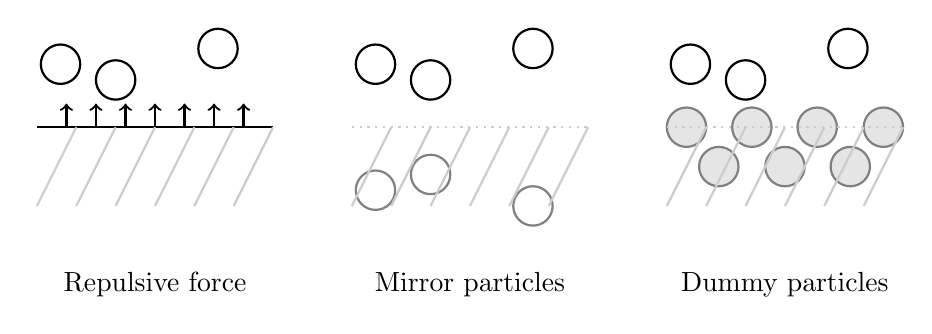
\begin{tikzpicture}[thick]
% Mathematical reflection
\draw (0.3,.8) circle (.25cm) node[pos=.5] (p0) {};
\draw (1,.6) circle (.25cm) node[pos=.5] (p1) {};
\draw (2.3,1) circle (.25cm) node[pos=.5] (p2) {};
\draw (0,0) -- (3,0);
\foreach \i in {1,...,6}{
	\draw[black!20] (.5*\i-.5,-1) -- (.5*\i,0);
}
% Forces
\foreach \i in {1,...,7}{
	\draw[->] (.375*\i,0) -- (.375*\i,.3);
}
\node at (1.5,-2) {Repulsive force};

% Mirror 
\draw (4.3,.8) circle (.25cm) node[pos=.5] (p0) {};
\draw (5,.6) circle (.25cm) node[pos=.5] (p1) {};
\draw (6.3,1) circle (.25cm) node[pos=.5] (p2) {};
\draw[black!50] (4.3,-.8) circle (.25cm) node[pos=.5] (mii1) {};
\draw[black!50] (5,-.6) circle (.25cm) node[pos=.5] (mii2) {};
\draw[black!50] (6.3,-1) circle (.25cm) node[pos=.5] (mii3) {};
\draw[black!20,dotted] (4,0) -- (7,0);
\foreach \i in {1,...,6}{
	\draw[black!20] (.5*\i-.5+4,-1) -- (.5*\i+4,0);
}
\node at (5.5,-2) {Mirror particles};

% Dummies
\draw[black!50,fill=black!10] (8.25,0) circle (.25cm) node[pos=.5] (d0) {};
\draw[black!50,fill=black!10] (9.08,0) circle (.25cm) node[pos=.5] (d1) {};
\draw[black!50,fill=black!10] (9.91,0) circle (.25cm) node[pos=.5] (d2) {};
\draw[black!50,fill=black!10] (10.75,0) circle (.25cm) node[pos=.5] (d3) {};
% second layer
\draw[black!50,fill=black!10] (8.66,-.5) circle (.25cm) node[pos=.5] (d4) {};
\draw[black!50,fill=black!10] (9.50,-.5) circle (.25cm) node[pos=.5] (d5) {};
\draw[black!50,fill=black!10] (10.33,-.5) circle (.25cm) node[pos=.5] (d6) {};
%\draw (1,-.25) circle (.25cm) node[pos=.5] (d4) {};
%normal parts
\draw (8.3,.8) circle (.25cm) node[pos=.5] (p0) {};
\draw (9,.6) circle (.25cm) node[pos=.5] (p1) {};
\draw (10.3,1) circle (.25cm) node[pos=.5] (p2) {};
\draw[dotted,black!20] (8,0) -- (11,0);
\foreach \i in {1,...,6}{
	\draw[black!20] (.5*\i-.5+8,-1) -- (.5*\i+8,0);
}
\node at (9.5,-2) {Dummy particles};
\end{tikzpicture}
\caption{Different boundaries condition methods}
\label{fig:SPH:boundaries}
\end{figure}

For this experiment, realistic boundaries conditions were needed. 
Several methods are possible with SPH we focused on the main ones, the repulsive wall, the mirror particles \cite{libersky1991smooth} and the dummies particles implementation \cite{adami2012generalized}. 
Those boundaries conditions implementation are presented in figure~\ref{fig:SPH:boundaries}.

For the current implementation, we used the dummies particles method.
The wall particles are just considered as normal particles, with specific equations, and their quantities are evolved during the run. 
The main difference is that their position does not evolve at the end of the step.
They are identified in the code with a specific type, provided during the data generation. 

\subsection{Astrophysics: neutron stars coalescence}

The final aim of our tests is to simulate astrophysical events. 
We are interested in one of the most important event recently discovered. 
Last year the Laser Interferometer Gravitational Wave, LIGO, detected the first gravitational wave generated by binary neutron stars merging \cite{abbott2017gw170817} and also more complexes event with Binary Black Holes coalescence in \cite{abbott2017gw170814}.


\subsubsection{Solving Lane-Emden Equation}

We need to determine the density function based on the radius. 

As we consider the star as a polytropic fluid, we use the equation of Lane-Emden which is a form of the Poisson equation: 

\begin{equation}\label{eq_LaneEmden}
  \frac{d^2\theta}{d \xi^2}+ \frac{2}{\xi}\frac{d\theta}{d\xi}+\theta^n = 0
\end{equation}

With $\xi$ and $\theta$ two dimensionless variables. 
There is only exact solutions for a polytropic index $n = 0.5$, $1$ and $2$.
In our work we use a polytropic index of $1$ which can correspond to a NS simulation.

For $n=1$ the solution of equation \ref{eq_LaneEmden} is: 

\begin{equation}
\theta(\xi)=\frac{sin(\xi)}{\xi}
\end{equation}

We note $\xi_1 = \pi$, the first value of $\xi$ as $\theta(\xi) = 0$.
$\theta(\xi)$ is also defined as: 
\begin{equation}
 \theta(\xi) = \Big(\frac{\rho(\xi)}{\rho_c}\Big)^{\frac{1}{n}}  = \frac{\rho(\xi)}{\rho_c}
\end{equation}

With $\rho_c$ the internal density of the star and $\rho$ the density at a determined radius. $\xi$ is defined as:  
$$ \xi = Ar = \sqrt{\frac{4\pi G}{K(n+1)}\rho_c^{(n-1)/n}} \times r = \sqrt{\frac{2\pi G}{K}}\times r \mbox{ (for } n=1 \mbox{)}$$

With $K$ a proportionality constant.

From the previous equations we can write the stellar radius $R$ as:
\begin{equation}
R = \sqrt{\frac{K(n+1)}{4\pi G}}\rho_c^{(1-n)/2}\xi_1 = \sqrt{ \frac{K}{2\pi G} } \times \xi_1
\end{equation} 

(We note that for $n=1$ the radius does not depend of the central density.)

If, for example, we use dimensionless units as $G=R=M=1$ (for the other results we use CGS with $G = 6.674 \times 10^{-8} cm^3g^{-1}s^{-2}$) 
We can compute K as: 
\begin{equation}
\label{eq:constant}
K = \frac{R^2  2 \pi G}{\xi_1^2}
\end{equation}

\begin{center}
\begin{tabular}{c|c|c|c|c|}
 & $NS_1$ & $NS_2$ & $NS_3$ & $NS_4$ \\ 
\hline 
Radius (cm) & $R=G=M=1$ & 1500000 & 1400000 & 960000 \\ 
\hline 
K & 0.636619 & 95598.00 & 83576.48 & 39156.94\\ 
\hline 
\end{tabular}
\end{center} 

Then we deduce the density function of $r$ as :

$$\rho(\xi) = \frac{sin(A\times r)}{A \times r} \times \rho_c \mbox{ with } A = \sqrt{\frac{2\pi G}{K}}
$$

As we know the total Mass $M$, the radius $R$ and the gravitational constant $G$ we can compute the central density as: 

$$ \rho_c = \frac{M A^3}{4 \pi (sin(AR)-ARcos(AR)) } $$

Then we normalize the results to fit $R = M = G = 1$: $K' = K/(R^2G) $, $m_i' = m_i/M $, $h_i' = h_i / R$, $\vec{x_i}' = \vec{x_i}/R$ 

\section{Conclusion}


\bibliographystyle{alpha}
\bibliography{\locpath/biblio/biblio_langford,\locpath/biblio/biblio_graph,\locpath/biblio/biblio_sph,\locpath/biblio/biblio_hpc}

\end{document}